\section{Auswertung}
\label{sec:Auswertung}

%\begin{figure}
%  \centering
%  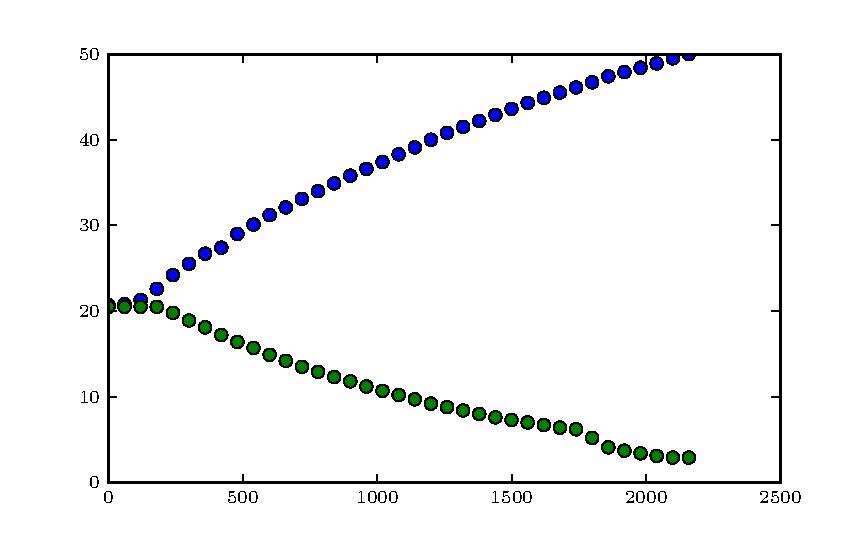
\includegraphics{plot.pdf}
%  \caption{Plot.}
%  \label{fig:plot}
%\end{figure}




%%%%%%%%%%%%%%%%%%%%%%%%%%%%%%%%%%%%%%
%Strömungsprofil
%%%%%%%Pumpleistung 70%
Zur Untersuchung der Streuintensität und der Momentangeschwindigkeit in Abhängigkeit zur Eindringtiefe ist es zunächst notwendig, die Eindringtiefe $x_{sec}$ welche in der Messung in Microsekunden aufgenommen wurde, in die Eindringtiefe $x_{m}$ in Millimetern umzurechnen.
Es werden hierzu zunächst die Verhältnisse zwischen $x_{sec}$ und $x_{m}$ für beide Materialien bestimmt.
\begin{figure}
  \centering
  \includegraphics{Bilder/f70.pdf}
  \caption{Plot.}
  \label{fig:f70}
\end{figure}
\begin{figure}
  \centering
  \includegraphics{Bilder/I70.pdf}
  \caption{Plot.}
  \label{fig:I70}
\end{figure}

\begin{table}
\centering
\caption{Pumpleistung 70\%}
\label{tab:pl70}
\begin{tabular}{ccccc}
  \toprule
  Eindringtiefe in sec & Eindringtiefe/$\si{\milli\meter}$ & $I_\mathrm{S}$/$\si{\square\volt\per\second}$ & $\Delta \nu$/$\si{\Hz}$ & momentane Geschwindigkeit/$\si{\meter\per\second}$ \\
\midrule
13.0 & 34.5 & 90.0 & 439.0 & 1.145 \\
13.5 & 35.4 & 114.0 & 490.0 & 1.278 \\
14.0 & 36.3 & 126.0 & 562.0 & 1.466 \\
14.5 & 37.2 & 140.0 & 623.0 & 1.625 \\
15.0 & 38.1 & 156.0 & 647.0 & 1.687 \\
15.5 & 39.0 & 160.0 & 623.0 & 1.625 \\
16.0 & 39.9 & 176.0 & 574.0 & 1.497 \\
16.5 & 40.8 & 187.0 & 500.0 & 1.304 \\
17.0 & 41.7 & 183.0 & 439.0 & 1.145 \\
17.5 & 42.6 & 206.0 & 421.0 & 1.098 \\
18.0 & 43.4 & 250.0 & 500.0 & 1.304 \\
18.5 & 44.3 & 495.0 & 500.0 & 1.304 \\
19.0 & 45.2 & 438.0 & 500.0 & 1.304 \\
19.5 & 46.1 & 348.0 & 500.0 & 1.304 \\
\bottomrule
\end{tabular}
\end{table}




%%%%%%%Pumpleistung 45%


\begin{figure}
  \centering
  \includegraphics{Bilder/f45-2.pdf}
  \caption{Plot.}
  \label{fig:f45}
\end{figure}
\begin{figure}
  \centering
  \includegraphics{Bilder/I45-2.pdf}
  \caption{Plot.}
  \label{fig:I45}
\end{figure}
\begin{table}
  \centering
  \caption{Pumpleistung 45\%}
  \label{tab:pl45}
  \begin{tabular}{ccccc}
  \toprule
Eindringtiefe in sec & Eindringtiefe/$\si{\milli\meter}$ & $I_\mathrm{S}$/$\si{\square\volt\per\second}$ & $\Delta \nu$/$\si{\Hz}$ & momentane Geschwindigkeit/$\si{\meter\per\second}$ \\
\midrule
13.0 & 34.5 & 90.0 & 220.0 & 0.574 \\
13.5 & 35.4 & 120.0 & 232.0 & 0.605 \\
14.0 & 36.3 & 155.0 & 269.0 & 0.702 \\
14.5 & 37.2 & 170.0 & 305.0 & 0.795 \\
15.0 & 38.1 & 180.0 & 317.0 & 0.827 \\
15.5 & 39.0 & 208.0 & 305.0 & 0.795 \\
16.0 & 39.9 & 230.0 & 281.0 & 0.733 \\
16.5 & 40.8 & 203.0 & 269.0 & 0.702 \\
17.0 & 41.7 & 196.0 & 232.0 & 0.605 \\
17.5 & 42.6 & 191.0 & 226.0 & 0.589 \\
18.0 & 43.4 & 232.0 & 244.0 & 0.636 \\
18.5 & 44.3 & 444.0 & 256.0 & 0.668 \\
19.0 & 45.2 & 360.0 & 244.0 & 0.636 \\
19.5 & 46.1 & 300.0 & 256.0 & 0.668 \\
\bottomrule
\end{tabular}
\end{table}
